\chapter{Controle de versões utilizando o Git}
\label{apendice_git}

Um sistema de controle de versões - ou configurações - é um sistema que fornece uma série de funcionalidades para controlar a evolução de um conjunto de arquivos. Entre essas funcionalidades estão ter acesso às versões anteriores de arquivos, controlar quem realizou uma determinada alteração e comparar versões com o intuito de analisar as diferenças.  Além disso, conforme Otte. \cite{otte2009version}, esses sistemas têm sido utilizados como uma ferramenta de backup, pois  permitem voltar a uma versão anterior caso algo esteja errado com a versão atual. O Git é um sistema moderno de controle de versão desenvolvido pelo também criador do Linux, Linus Torvalds. Conforme Loeliger et al.\cite{loeliger2012version}, ele pode ser visto como uma evolução de sistemas mais antigos como o CVS\cite{vesperman2006essential} e o Subversion\cite{pilato2008version}. 

O principal diferencial do Git em relação aos outros sistemas de versionamento é a sua característica distribuída. O Git foi projetado para funcionar muito bem em contextos onde exista uma grande quantidade de pessoas interagindo com o mesmo projeto e, ainda assim, haja a necessidade que essa interação ocorra de uma forma organizada e rastreável. Essa característica distribuída é alcançada por meio de alguns recursos:

\begin{itemize}
\item \textbf{Facilidade para a realização de cópias de um repositório}. Qualquer pessoa no mundo pode realizar uma cópia local de um repositório de arquivos público gerenciado por uma instância do sistema Git. Para isso, basta instalar uma versão do Git no computador local e utilizar o comando \textit{clone} seguido pela URL do repositório. \textbf{A cópia obtida contém todo o histórico do projeto como também todos os arquivos necessários para que o versionamento possa ser realizado}. Isso faz com que não exista obrigatoriamente um único repositório central de um determinado projeto. Cada cópia é um repositório independente. 

\item \textbf{É extremamente eficiente comparado às alternativas anteriores.} Uma das razões para essa eficiência está na estratégia utilizado para realizar o controle das versões dos arquivos. No Git existe uma pasta chamada \textit{.git} na pasta onde estão os arquivos sendo gerenciados. Essa pasta contém todos os dados referentes ao histórico dos arquivos como também todas as informações necessárias para realizar o controle de versão. Dessa forma, o Git não precisa acessar à rede para buscar alguma informação necessária para o controle de versão. Todos os dados estão no próprio sistema de arquivos usado para armazenar os arquivos gerenciados. Outra razão da eficiência do Git é a inexistência de um processo que necessariamente precisa estar em execução para que o controle de versão funcione. Isso era necessário nos sistemas anteriores como é o caso do Subversion. Nele havia um \textit{daemon} responsável por realizar o versionamento de arquivos. No Git isso não ocorre. Em vez disso, o Git fornece um conjunto de programas que ao serem executados conseguem realizar as alterações necessárias nos arquivos de controle de versionamento. 

\end{itemize}


O funcionamento do Git é baseado em um grafo em que cada nó  representa uma versão dos arquivos. Um exemplo dessa organização pode ser visto na Figura \ref{fig:cap_experimento_exemplo_grafo_git}. Nela, um repositório foi iniciado pelo \textit{commit} $C1$ e depois houve uma alteração por meio do \textit{commit} $C2$. Nesse ponto, foram criadas duas novas \textit{branches}. Uma \textit{branch} é um fluxo independente de versões. Normalmente, a \textit{branch} principal de um repositório Git é chamada de master. No exemplo apresentado, os \textit{commit}  $C4$ e $C6$ foram criados a partir do commit $C2$ da \textit{branch} principal. Porém, tanto eles quanto o \textit{commit} $C3$ são totalmente independentes e podem apresentar conteúdos diferentes. Ainda assim, essas linhas independentes de evolução, podem novamente ser combinadas por meio do que é chamado de \textit{merge}. Na Figura \ref{fig:cap_experimento_exemplo_grafo_git_merge}  temos o resultado do \textit{merge} realizado entre as \textit{branches} master e a \textit{branch} 1. A versão obtida após o commit $C8$ contém tanto as alterações que foram realizadas nos \textit{commits} $C4$ e $C5$ quanto as alterações realizadas no commit $C3$. Entretanto, essa operação não traz nenhum impacto à \textit{branch 2}. A criação de \textit{commits}, \textit{branches}, \textit{merges} e todas as outras ações necessárias para o versionamento dos arquivos em um repositório Git são realizados por meio de comandos que esse sistema disponibiliza. Para extrairmos as informações dos projetos analisados nesta pesquisa, utilizaremos alguns desses comandos.  Na Apêndice \ref{ape:comandos_git} há uma lista com os principais deles e quais as suas funções.  

 \begin{figure}[H]
  \centering
  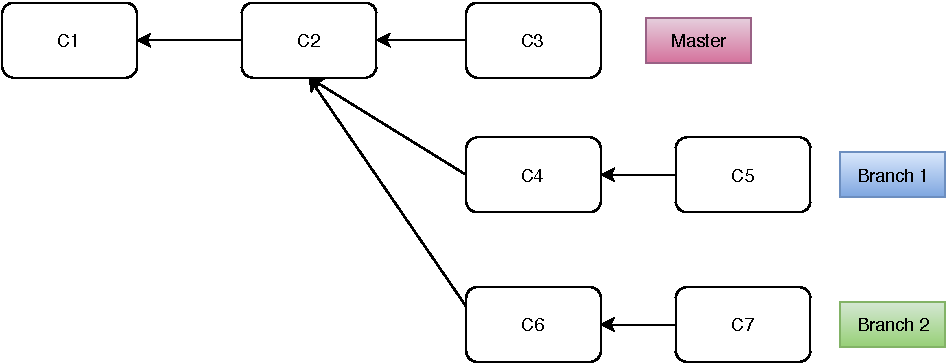
\includegraphics{capitulo_estudo_caso/exemplo_grafo_git.pdf} 
  \caption{Exemplo da estrutura de armazenamento de versões do Git.}
  \label{fig:cap_experimento_exemplo_grafo_git} 
\end{figure}

 \begin{figure}[H]
  \centering
  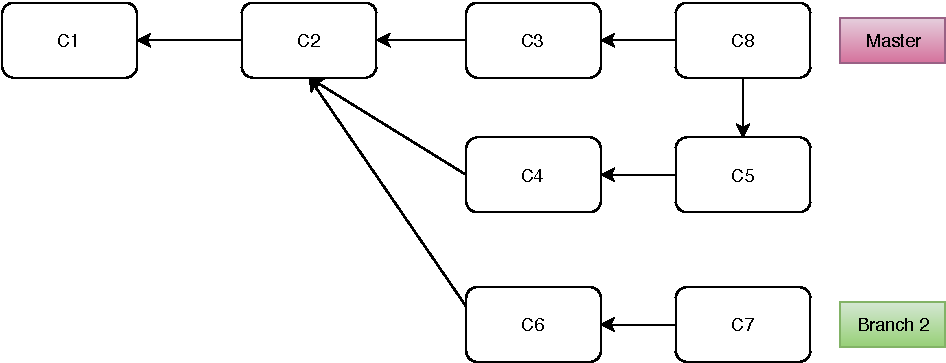
\includegraphics{capitulo_estudo_caso/exemplo_grafo_git_merge.pdf} 
  \caption{Exemplo de merge entre duas \textit{branches}.}
  \label{fig:cap_experimento_exemplo_grafo_git_merge} 
\end{figure}


\section{Comandos Git}
\label{ape:comandos_git}


A Tabela \ref{table:comandos_git} apresenta uma lista com os principais comandos do git.

\begin{table}[H]
\label{table:comandos_git}
\centering
\def\arraystretch{2.5}%
\begin{tabular}{|c|c|c|}
\hline
Comando & \pbox{6cm}{Descrição}                                                     & Exemplo                                     \\ \hline
clone   & \pbox{6cm}{Realiza uma cópia local de um repositório remoto }             & clone https://github.com/torvalds/linux.git \\ \hline
add     & \pbox{6cm}{Inclui um ou mais arquivos no gerenciamento de versão}         & add file.txt                                \\ \hline
commit  &\pbox{6cm} {Efetiva no histórico as mudanças realizadas}                   & commit -m ``History message"                 \\ \hline
push    & \pbox{6cm}{Envia as alterações locais para um repositório remoto}         & git push -u origin branch                   \\ \hline
pull    & \pbox{6cm}{Atualiza os arquivos locais com base em um repositório remoto} & git pull                                    \\ \hline
merge    & \pbox{6cm}{Realiza o merge entre duas \textit{branches}} & merge branch1                                 \\ \hline
branch    & \pbox{6cm}{Cria uma nova branch} & branch branch3                                 \\ \hline
checkout    & \pbox{6cm}{Muda o diretório de trabalho atual para uma determinada branch} & checkout branch3                                 \\ \hline
\end{tabular}
\caption{Comandos básicos do GIT.}
\label{table:comandos_git}
\end{table}

